\documentclass[11pt]{aghdpl}
% \documentclass[en,11pt]{aghdpl}  % praca w języku angielskim

% Lista wszystkich języków stanowiących języki pozycji bibliograficznych użytych w pracy.
% (Zgodnie z zasadami tworzenia bibliografii każda pozycja powinna zostać utworzona zgodnie z zasadami języka, w którym dana publikacja została napisana.)
\usepackage[english,polish]{babel}

% Użyj polskiego łamania wyrazów (zamiast domyślnego angielskiego).
\usepackage{polski}

\usepackage[utf8]{inputenc}

% dodatkowe pakiety

\usepackage{mathtools}
\usepackage{amsfonts}
\usepackage{amsmath}
\usepackage{amsthm}
\usepackage{rotating}
\usepackage{elm-highlighting}
\usepackage{parcolumns}
\usepackage{js-highlighting}
\usepackage[section]{placeins}

% --- < bibliografia > ---

\usepackage[
style=numeric,
sorting=none,
language=autobib,
autolang=other,
urldate=iso8601,
backref=false,
isbn=true,
url=false,
maxbibnames=3,
backend=biber
]{biblatex}

%
% Zastosuj styl wpisu bibliograficznego właściwy językowi publikacji.
%language=autobib,
%autolang=other,
% Zapisuj datę dostępu do strony WWW w formacie RRRR-MM-DD.
%urldate=iso8601,
% Nie dodawaj numerów stron, na których występuje cytowanie.
%backref=false,
% Podawaj ISBN.
%isbn=true,
% Nie podawaj URL-i, o ile nie jest to konieczne.
%url=false,
%
% Ustawienia związane z polskimi normami dla bibliografii.
%maxbibnames=3,
% Jeżeli używamy BibTeXa:
%backend=bibtex
%]{biblatex}

\usepackage{csquotes}
% Ponieważ `csquotes` nie posiada polskiego stylu, można skorzystać z mocno zbliżonego stylu chorwackiego.
\DeclareQuoteAlias{croatian}{polish}

\addbibresource{bibliografia.bib}

% Nie wyświetlaj wybranych pól.
%\AtEveryBibitem{\clearfield{note}}


% ------------------------
% --- < listingi > ---

% Użyj czcionki kroju Courier.
\usepackage{courier}

\usepackage{listings}
\lstloadlanguages{TeX}

\lstset{
	literate={ą}{{\k{a}}}1
           {ć}{{\'c}}1
           {ę}{{\k{e}}}1
           {ó}{{\'o}}1
           {ń}{{\'n}}1
           {ł}{{\l{}}}1
           {ś}{{\'s}}1
           {ź}{{\'z}}1
           {ż}{{\.z}}1
           {Ą}{{\k{A}}}1
           {Ć}{{\'C}}1
           {Ę}{{\k{E}}}1
           {Ó}{{\'O}}1
           {Ń}{{\'N}}1
           {Ł}{{\L{}}}1
           {Ś}{{\'S}}1
           {Ź}{{\'Z}}1
           {Ż}{{\.Z}}1,
	basicstyle=\footnotesize\ttfamily,
}

% ------------------------

\AtBeginDocument{
	\renewcommand{\tablename}{Tabela}
	\renewcommand{\figurename}{Rys.}
}

% ------------------------
% --- < tabele > ---

\usepackage{array}
\usepackage{tabularx}
\usepackage{multirow}
\usepackage{booktabs}
\usepackage{makecell}
\usepackage[flushleft]{threeparttable}

\usepackage{fancyref}

% defines the X column to use m (\parbox[c]) instead of p (`parbox[t]`)
\newcolumntype{C}[1]{>{\hsize=#1\hsize\centering\arraybackslash}X}


%---------------------------------------------------------------------------

\author{Kamil Osuch}
\shortauthor{K. Osuch}

\titlePL{Porównanie budowania i rozwoju aplikacji WWW w języku Elm i~technologiach React+Redux}
\titleEN{Comparision of building and development of web application in Elm language and React+Redux technologies}


\shorttitlePL{Porównanie budowania i rozwoju aplikacji WWW w języku Elm i~technologiach React+Redux} % skrócona wersja tytułu jeśli jest bardzo długi
\shorttitleEN{Comparision of building and development of web application in Elm language and React+Redux technologies}

\thesistype{Praca dyplomowa inżynierska}
%\thesistype{Master of Science Thesis}

\supervisor{dr inż. Piotr Matyasik}
%\supervisor{Marcin Szpyrka PhD, DSc}

\degreeprogramme{Informatyka}
%\degreeprogramme{Computer Science}

\date{2017}

\department{Katedra Informatyki Stosowanej}
%\department{Department of Applied Computer Science}

\faculty{Wydział Elektrotechniki, Automatyki,\protect\\[-1mm] Informatyki i Inżynierii Biomedycznej}
%\faculty{Faculty of Electrical Engineering, Automatics, Computer Science and Biomedical Engineering}

\acknowledgements{Serdecznie dziękuję mojemu promotorowi za cierpliwość, a także rodzinie i znajomym, którzy musieli znosić moje zachowanie w czasie tworzenia tej pracy}


\setlength{\cftsecnumwidth}{10mm}

%---------------------------------------------------------------------------
\setcounter{secnumdepth}{4}
\brokenpenalty=10000\relax

\begin{document}

\titlepages

% Ponowne zdefiniowanie stylu `plain`, aby usunąć numer strony z pierwszej strony spisu treści i poszczególnych rozdziałów.
\fancypagestyle{plain}
{
	% Usuń nagłówek i stopkę
	\fancyhf{}
	% Usuń linie.
	\renewcommand{\headrulewidth}{0pt}
	\renewcommand{\footrulewidth}{0pt}
}

\setcounter{tocdepth}{2}
\tableofcontents
\clearpage

\chapter{Wprowadzenie} \label{chap:wprowadzenie}

W ciągu ostatnich kilku lat sposób tworzenia stron internetowych przechodził intensywne i szybkie zmiany. W związku z rosnącą popularnością internetu na całym świecie okazało się, że zwykłe, proste strony internetowe nie są wystarczające. W związku z tym szybko one awansowały ze statycznych dokumentów hipertekstowych jedynie wyświetlających zawartość użytkownikowi, do poziomu aplikacji internetowych, z którymi może on wejść w interakcję, a nawet używać ich dokładnie tak samo, jak programów zainstalowanych w swoim systemie operacyjnym. 

Rynek tworzenia oprogramowania webowego został przejęty głównie przez język JavaScript nazywany dziś przez niektórych asemblerem stron internetowych \cite{JSAssembly}. Coraz większe wymagania co do działania stron internetowych spowodowały, że tworzenie stron bezpośrednio w JavaScript'cie stało się zbyt skomplikowane i niewystarczające. Z pomocą przychodzą biblioteki, frameworki oraz języki kompilowane do JavaScriptu. Upraszczają one tworzony kod, często zmieniając też jego strukturę. Dzięki temu umożliwiają korzystanie z gotowych funkcjonalności w prosty i wygodny sposób. Przykładami tutaj mogą być biblioteki takie jak jQuery, Angular, React, Redux, czy Ember.js. 

W przypadku języków kompilowanych do JavaScriptu zmiany są jeszcze większe. Programista nie zastanawia się nad tym, że ostateczna wersja stworzonego przez niego programu jest zapisana w zupełnie innym języku. Przykładami takich języków są chociażby CoffeeScript, TypeScript czy Elm.

Ilość takich rozwiązań tworzy nieograniczoną liczbę podejść do tworzenia aplikacji webowych, a ich liczba każdego dnia rośnie. W związku z tym powstaje wiele artykułów porównujących różne podejścia, zarówno pod względami architektury kodu, jak i szybkości działania samych aplikacji.

Celem niniejszej pracy jest porównanie budowania i rozwoju aplikacji webowych przy pomocy języka Elm, oraz kombinacji bibliotek React.js i Redux. Technologie te zostaną szczegółowo porównane pod względem dostępnych funkcjonalności, szybkości działania aplikacji, dostępności bibliotek oraz trudności zarówno w tworzeniu pierwszej wersji aplikacji, jak i rozwoju istniejącego już kodu.

Wybór tematu pracy był podyktowany przede wszystkim poszukiwaniem alternatywnych rozwiązań służących do tworzenia aplikacji webowych. Biblioteki takie jak React czy Redux zdominowały rynek, przez co ilość wykorzystywanych sposobów budowania stron internetowych w stosunku do ilości dostępnych możliwości jest bardzo mała.

Ważną częścią pracy jest próba implementacji w języku Elm części projektu stworzonego przy pomocy kombinacji Reacta i~Reduxa. Pozwoli to na praktyczną możliwość analizy obu rozwiązań i wyspecyfikowanie napotkanych problemów.

W rozdziale \ref{chap:teoria} zostały krótko opisane charakterystyka języka JavaScript oraz podstawowe pojęcia związane z tworzeniem aplikacji webowych. Następnie krótko zostały opisane biblioteki React i Redux oraz język Elm.
Rozdział \ref{chap:porownanie} skupia się na porównaniu architektury obu rozwiązań, zwracając uwagę zarówno na funkcjonalności, które są dostępne domyślnie jednocześnie Elmie oraz kombinacji Reacta i~Reduxa, jak i na te rozwiązania, które domyślnie oferuje tylko jedna ze stron.
W rozdziale \ref{chap:tools} opisane zostały narzędzia, które są oferowane przez oba porównywane rozwiązania, ich możliwości, ograniczenia, a także poziom trudności ich użycia.
Rozdział \ref{chap:implementacja} opisuje założenia implementacji projektu tworzonego w ramach pracy, oraz problemy napotkane podczas próby stworzenia aplikacji, domyślnie napisanej za pomocą Reacta i Reduxa, przy pomocy języka Elm.
Rozdział \ref{chap:podsumowanie} zawiera krótkie podsumowanie przeprowadzonej analizy porównawczej. Opisuje on wnioski oraz możliwości rozwoju pracy.

\chapter{Podstawy teoretyczne} \label{chap:teoria}
W tym rozdziale zostaną omówione podstawowe pojęcia związane z tematem pracy. Pierwsze dwa podrozdziały skupiają się na opisie czym w ogóle jest aplikacja internetowa, oraz opisują jedno z najpopularniejszych podejść do budowania aplikacji internetowej, SPA. W kolejnych podrozdziałach zostały opisane technologie, które są porównywane w dalszej części pracy.
\section{Aplikacja internetowa}
Aplikacja internetowa jest czymś więcej niż zwykłą stroną internetową. Z definicji jest to aplikacja typu klient-serwer, w której klient jest uruchamiany przy pomocy przeglądarki internetowej. Oprogramowanie klienta jest pobierane na komputer klienta podczas wizyty na odpowiedniej stronie internetowej, przy użyciu standardowych procedur, takich jak HTTP. Aktualizacje oprogramowania klienta mogą odbywać się za każdym razem, gdy odwiedzana jest strona internetowa. W czasie trwania sesji przeglądarka internetowa interpretuje i wyświetla strony, oraz działa jako uniwersalny klient dla dowolnej aplikacji internetowej.
\begin{figure}[h]
	\centering
	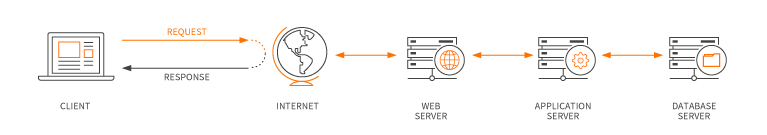
\includegraphics[width=\textwidth]{images/how_web_application_works}
	\caption{Podstawowy schemat działania aplikacji internetowej \cite{MaxCdnWebApp}}
\end{figure}
%\subsection{Krótki rys historyczny}
\section{SPA}Skrót SPA pochodzi od \textit{Single-page Application}. Jest to aplikacja internetowa działająca wewnątrz przeglądarki, która podczas użytkowania strony nie wymaga odświeżania strony. W tym podejściu, cały niezbędny kod źródłowy --- HTML, JavaScript i CSS --- jest pobierany przy pojedyńczym załadowaniu strony, lub odpowiednie zasoby są ładowane dynamicznie i dodawane do strony jedynie wtedy, kiedy jest to potrzebne. Idea jaka stoi za takim rozwiązaniem, to przede wszystkim lepszy, bardziej naturalny user expierience. Użytkownik po wejściu na stronę, nie musi przy każdej interakcji oczekiwać na ponowne załadowanie się strony, czy też jej odświeżanie.


\begin{figure}[!h]
	\centering
	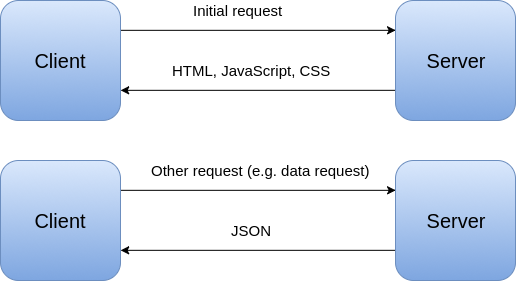
\includegraphics[width=0.6\textwidth]{images/spa}
	\caption{Podstawowy cykl życia SPA}
\end{figure}

Choć koncept SPA zaczął być częściej używany po spopularyzowaniu AJAX'a\footnote{Asynchronous JavaScript And XML}, to tak naprawdę dopiero od kilku lat jest on powszechnie wykorzystywany podczas budowania aplikacji internetowych. Serwisy takie jak Gmail, Google Maps, Twitter czy GitHub są właśnie aplikacjami typu single-page application. Także większość najpopularniejszych bibliotek JavaScript'owych umożliwiają implementację aplikacji internetowej zgodnie z zasadami SPA.
\subsection{Zalety}
\begin{itemize}
	\item Szybkość działania -- większość zasobów jest ładowana tylko raz podczas cyklu życia aplikacji, jedynymi informacjami, które są wymieniane z serwerem cały czas, są dane
	\item Brak ciągłego przeładowywania strony
	\item Znacznie prostszy proces wdrożenia aplikacji -- jedyne co jest potrzebne to statyczny serwer serwujący minimalnie 3 pliki -- pojedynczą stronę HTML, oraz 2 pakiety: jeden zawierający wszystkie style, drugi skupiający w sobie cały kod JavaScriptu
	\item Odciążenie strony serwerowej -- serwer, zamiast generować za każdym razem pełny kod strony, transmituje jedynie potrzebne w danej chwili dane
\end{itemize}
\subsection{Wady}
\begin{itemize}
	\item Powolne początkowe uruchomienie strony -- wymaga ono załadowania frameworku, oraz przynajmniej części aplikacji, która później już nie jest ponownie ściągana.
	\item Ze względu na zależność SPA od JavaScriptu, bardzo łatwo o pojawienie się wycieków pamięci pomiędzy długimi okresami czasu między przeładowaniami strony
\end{itemize}

\section{JavaScript}
JavaScript jest to wysokopoziomowy, słabo typowany, wieloparadgymatowy, skryptowy i interpretowany język programowania stworzony w 1995 roku przez Brendana Eicha dla firmy Netscape.  W roku 1997 organizacja Ecma International wydała na podstawie JavaScriptu standard języka skryptowego nazwany ECMAScript, na którym bazowanych jest większość silników JavaScript'owych.

JavaScript jest jedną z trzech głównych technologii wykorzystywanych przy tworzeniu treści związanych z siecią internetową. Obecnie 94,9\% spośród 10 milionów najbardziej popularnych stron internetowych wykorzystuje JavaScript (stan na grudzień 2017 \cite{JSUsage}).

\section{React.js}
React jest biblioteką języka JavaScript, wykorzystywaną do tworzenia graficznych interfejsów użytkownika. Pozwala ona na tworzenie rozbudowanych aplikacji internetowych, które używają danych i~mogą zmieniać swoją zawartość w czasie bez ponownego ładowania strony. Biblioteka została stworzona przez jednego z programistów Facebooka, Jordana Walke, który zainspirował się rozszerzeniem języka PHP, XHP, także stworzonym przez Facebooka. Pierwsze wersje biblioteki zostały użyte w 2011 roku na stronie aktualności Facebooka, a od 2012 roku jest ona wykorzystywana w~serwisie Instagram. Od 2013 roku React stał się wolnym oprogramowaniem, co spowodowało nagły wzrost jego popularności, a także umożliwiło społeczności  pomoc w rozwoju oprogramowania.

Ze względu na ogromny wpływ rynku urządzeń mobilnych, Facebook ogłosił w 2015 roku bibliotekę React Native, pozwalającą na korzystanie z architektury Reacta podczas budowania aplikacji mobilnych. To co wyróżniało tę bibliotekę od dotychczasowych sposobów tworzenia mobilnego oprogramowania, to brak konieczności powielania funkcjonalności dla każdej platformy z osobna. React Native pozwalał na wykorzystanie tego samego kodu źródłowego zarówno w aplikacji dla systemu Android jak i iOS.

Obecnie React jest jedną z najpopularniejszych bibliotek służących do tworzenia aplikacji internetowych. Jest wykorzystywany w ogromnej ilości znanych serwisów takich jak Facebook, Instagram, Spotify, Netflix czy eBay. 
\section{Redux}
Redux jest biblioteką języka JavaScript o otwartym kodzie źródłowym zaprojektowaną do zarządzania stanem aplikacji. Została stworzona w 2015 roku przez Dana Abramova. Działanie Reduxa może być opisane przez trzy zasady \cite{reduxDocs}:
\begin{enumerate}
	\item Istnieje jedno źródło prawdy -- stan całej aplikacji jest przechowywany w pojedyńczym obiekcie, który przechowuje całe drzewo stanu aplikacji.
	\item Stan służy tylko do odczytu -- jedynym sposobem na zmianę stanu jest wysłanie akcji -- obiektu opisującego co się stało, zwykle zawierającego typ akcji, oraz ewentualne dane, które mają wpływ na zmianę stanu.
	\item Zmiany stanu są dokonywane przy użyciu czystych funkcji -- aby określić, w jaki sposób drzewo stanu jest modyfikowane przez akcje, tworzy się funkcje zwane \textit{reducerami}, przyjmujące poprzedni stan i akcję jako argumenty, a zwracające nowy stan.
\end{enumerate}
\begin{figure}[h]
	\centering
	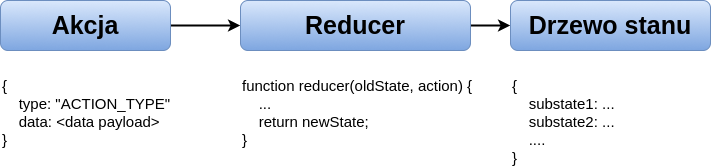
\includegraphics[width=0.9\textwidth]{images/redux_flow}
	\caption{Schemat działania Reduxa}
\end{figure}

\section{Elm}
Elm jest funcyjnym językiem programowania kompilowanym do JavaScriptu. Język został stworzony w 2012 roku przez Evana Czaplickiego, w ramach jego pracy dyplomowej. Na dalszy rozwój języka pozwoliła firma Prezi, która w 2013 roku zatrudniła twórcę języka. W 2016 roku Czaplicki zmienił firmę na NoRedInk i postanowił stworzyć organizację non-profit --- Elm Software Foundation --- której celem ma być promowanie, ochrona i rozwój języka Elm, oraz wszelka pomoc społeczności programistów tworzących oprogramowanie w Elmie \cite{newAdventures}.

Evan Czaplicki twierdzi, że jego język może konkurować z projektami takimi jak React, jako narzędzie do tworzenia aplikacji internetowych. Język kładzie bardzo duży nacisk na prostotę, łatwość użycia i jakość narzędzi \cite{elmGuide}.
\chapter{Porównanie architektury} \label{chap:porownanie}
Choć porównywanie kombinacji bibliotek z językiem programowania wydaje się dziwne, to jeżeli spojrzy się na funkcjonalności oferowane przez Reacta i Reduxa w porównaniu do możliwości Elma, można zauważyć pewne podobieństwa w sposobie budowania aplikacji. W tym rozdziale zostały opisane funkcjonalności, które są oferowane przez oba rozwiązania, oraz różnice występujące między Reactem i~Reduxem a Elmem dla każdej z funkcjonalności.

\section{Virtual DOM i składnia}
\subsection{Document Object Model}
DOM \footnote{z. ang. Document Object Model} jest niezależnym od platformy i języka programowania interfejsem, który pozwala programom i skryptom na dynamiczny dostęp i aktualizację treści, struktury i stylu dokumentu. Kiedy strona internetowa jest ładowana, przeglądarka tworzy DOM strony, będący obiektową reprezentacją dokumentu HTML. Służy ona jako interfejs umożliwiający pobieranie oraz modyfikację elementów HTML, które w DOM-ie są zdefiniowane jako obiekty.

\subsection{Dlaczego DOM jest powolny?}
Każda akcja na stronie powoduje zmianę DOM-u. Ze względu na jego drzewiastą strukturę, sama modyfikacja DOM-u jest szybka. Jednak każdy z modyfikowanych elementów oraz wszystkie jego dzieci muszą dodatkowo przejść przez dwa kosztowne etapy:
\begin{enumerate}
	\item Reflow będący procesem, podczas którego przeliczane zostają wymiary oraz pozycja elementu. Dokładnie ten sam proces jest uruchamiany na węzłach dzieci, a także elementach, które pojawiają się w DOM-ie później niż główny element. Reflow jest kosztowny, ponieważ zmiana pojedynczego elementu w strukturze DOM-u może spowodować wywołanie Reflow na wielu innych elementach.
	\item Repaint, w którym niektóre partie ekranu muszą zostać zaktualizowane, czy to ze względu na modyfikacje wymiarów i~pozycji elementu, czy przez zmiany stylistyczne, takie jak zmiana koloru tła. Etap ten jest kosztowny ponieważ przeglądarka musi sprawdzić widoczność innych węzłów w~DOM-ie.
\end{enumerate} 

\subsection{Virtual DOM}
Virtual DOM jest to lekka, niezależna od przeglądarki abstrakcyjna reprezentacja DOM-u. Służy ona między innymi do zminimalizowania kosztu stworzonego przez etapy Reflow i Repaint. Zamiast tworzyć za każdym razem drzewo składające się z węzłów DOM-u, Virtual DOM pozwala na stworzenie tego drzewa przy pomocy abstrakcyjnych węzłów, które są odpowiednikami faktycznych elementów DOM-u. Dzięki temu wszystkie operacje modyfikujące widok mogą być wykonane na abstrakcyjnej strukturze, a dopiero końcowy rezultat powoduje modyfikację faktycznego DOM-u.

\subsection{Algorytm porównywania różnic}
Koncepcja Virtual DOM-u została wykorzystana do tego, aby w każdej klatce budować zupełnie nową scenę. Choć taka operacja wydaje się kosztowna, to tak naprawdę zbudowanie pełnego drzewa Virtual DOM-u jest szybkie, i jest wykorzystywane przy każdej aktualizacji widoku. W momencie gdy następuje zmiana powodująca modyfikację widoku, algorytm porównuje ze sobą stare i nowe drzewo Virtual DOM-u. Wszystkie komponenty, w których nastąpiła jakakolwiek zmiana są oznaczane specjalną flagą, która określa, że dany węzeł został zmodyfikowany. Na tej podstawie budowana jest dokładna lista zmian jakie nastąpiły w widoku. Następnie lista ta jest wykorzystywana do modyfikacji faktycznego DOM-u, lecz nie jako pojedynczo wprowadzane zmiany, a jedna aktualizacja drzewa dokumentu. 

\begin{figure}[h]
	\centering
	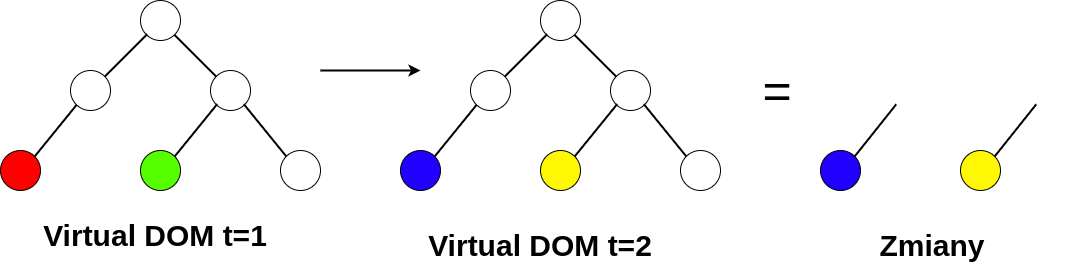
\includegraphics[width=0.8\textwidth]{images/diff_algorithm}
	\caption{Schemat działania algorytmu  porównywania różnic}
	\label{fig:diffAlgorithm}
\end{figure}

\subsection{Reprezentacja w Elmie}
Zarówno React, jak i Elm posiadają własne implementacje Virtual DOM-u. W Elmie abstrakcyjną reprezentację węzła otrzymujemy przy pomocy funkcji \lstinline{node}, która jako atrybuty przyjmuje tag, listą atrybutów HTML, oraz listę węzłów dzieci:
\begin{lstlisting}[style=elm-style]
	node : String -> List Attrbiute -> List Html -> Html
\end{lstlisting}
W przypadku użycia tagów HTML, takich jak \lstinline{div}, Elm udostępnia funkcje pomocnicze, które posiadają już uzupełniony atrybut tag, pozostawiając nam do określenia atrybuty węzła oraz jego dzieci. Elm nie ma specjalnej składni, która służyłaby do budowania widoków. Wszystkie elementy, z których budowany jest widok aplikacji, są funkcjami. W przypadku budowania widoku jedynym wymaganiem jest, aby funkcja go budująca zwracała rekord specjalnego typu \lstinline[style=elm-style]{Html msg}, który jest głównym blokiem służącym do tworzenia wyjściowego kodu HTML.

\subsection{Reprezentacja w React}
W przypadku Reacta mamy do czynienia ze znacznie bardziej rozszerzonym podejściem.  Bazowym elementem reprezentującym abstrakcyjny węzeł Virtual DOM-u jest ReactElement. Analogicznie jak w przypadku funkcji \lstinline{node} w Elmie jest to obiekt posiadający informację o tagu, który reprezentuje, atrybutach zdefiniowanego węzła, oraz listę dzieci. Przykład tworzenia takiego elementu można zobaczyć we fragmencie kodu \ref{listing:jsreactelement}. 

\begin{minipage}{.45\textwidth}
	\begin{lstlisting}[caption=Javascript,style=JavaScript,label = listing:jsreactelement]
	var divHello = React.createElement(
	"div",
	{ className: "myclass" },
	"Hello world!"
	);
	\end{lstlisting}
\end{minipage}\hfill
\begin{minipage}{.45\textwidth}
	\begin{lstlisting}[caption=JSX,style=JavaScript,firstnumber=1,label = listing:jsx]
	var divHello = (
	<div className="myclass">
		Hello world!
	</div>
	);
	\end{lstlisting}
\end{minipage}

\subsection{Test wydajnościowy}
Biorąc pod uwagę to, że każdy element Virtual DOM-u w React'cie jest zbudowany w podobny sposób, można zauważyć, że w przypadku rozbudowanej aplikacji, kod bardzo szybko staje się skomplikowany i niezrozumiały. Aby tego uniknąć, Facebook stworzył specjalne rozszerzenie składni dla JavaScriptu -- JSX. Z wyglądu przypomina składnię języka HTML, lecz zasadniczo dostarcza cukier syntaktyczny dla funkcji \lstinline[style=JavaScript]{createElement}. Fragmenty kodu \ref{listing:jsx} oraz \ref{listing:jsreactelement} są dokładnie tymi samymi wyrażeniami, z tą różnicą, że w drugim przypadku został wykorzystany JSX. Takie podejście pozwala na użycie JSX-a wewnątrz instrukcji JavaScriptu, przypisywanie go do zmiennych, czy też zwracanie z funkcji. Operacja zachodzi także w drugą stronę, co znaczy, że można korzystać z kodu JavaScriptu wewnątrz składni JSX-a. Taki kod musi być objęty nawiasami klamrowymi, aby odróżnić fragmenty napisane w JavaScript'cie od kodu JSX-a. 

% Test czasu renderowania
Choć główne założenia Virtual DOM-u w Elmie i React'cie są podobne, to jego implementacje nie są identyczne, w związku z czym można je porównać pod względem wydajnościowym. W tym przypadku wykorzystany został test wydajnościowy stworzony przez twórcę Elma \cite{perComp}. Pozwala on na porównanie czasu renderowania różnych implementacji aplikacji TodoMVC. Jest to prosty projekt listy zadań, umożliwiający dodawanie i usuwanie wpisów, oznaczanie ich jako zakończone, a także odfiltrowywanie na podstawie statusu wpisów. Test zakłada realistyczny scenariusz, w którym każda zmiana jest wyświetlona jako pojedyncza klatka, tak jakby to faktyczny użytkownik przeprowadzał test. Algorytm scenariusza wykonywany w trakcie pomiaru średniego czasu renderowania wygląda następująco:
\begin{enumerate}
	\item Stworzenie strony niezawierającej wpisów
	\item Dodanie 100 wpisów do listy
	\item Oznaczenie każdego z elementów jako zakończony
	\item Usunięcie wszystkich wpisów
\end{enumerate}
Dodatkowo zostały przyjęte następujące założenia, które sprawiają, że przeprowadzony test jest sprawiedliwy:
\begin{enumerate}
	\item Brak zgrupowanych zdarzeń -- oznacza to, że zamiast generować zdarzenia w pojedynczej pętli, algorytm tworzy jedno zdarzenie na raz, przechodząc do następnego dopiero po wyrenderowaniu całego widoku. Gdyby takie założenie nie zostało przyjęte, to przykładowo w przypadku dodawania wpisów, zmiany następowałyby na tyle szybko, że zamiast wyświetlić 100 klatek, przeglądarka wyświetliłaby tylko jedną.
	\item Brak użycia \lstinline{requestAnimationFrame} -- funkcja ta informuje przeglądarkę o zamiarze wykonania animacji i żąda od przeglądarki wywołania określonej funkcji w celu odświeżenia animacji przed następną zmianą w widoku. Oznacza to, że odświeżenie animacji jest wyrównane do 60 razy na sekundę, niezależnie od tego, jak wiele klatek wygeneruje JavaScript. Elm wykorzystuje tą funkcję do pomijania części klatek, które i tak nie będą widoczne dla użytkownika. W z związku z realistycznym scenariuszem, oraz brakiem podobnej optymalizacji w innych implementacjach, funkcja ta musiała zostać usunięta z Elma w ramach przeprowadzanego testu.
\end{enumerate}

\begin{figure}[h]
	\centering
	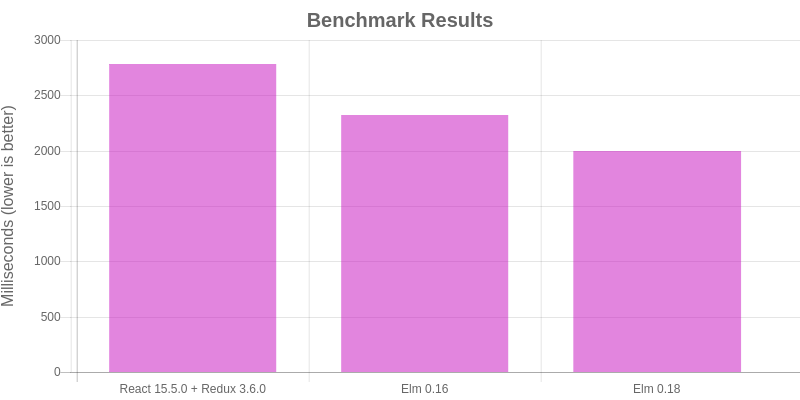
\includegraphics[width=0.9\textwidth]{images/render_comparision}
	\caption{Porównanie czasu renderowania aplikacji TodoMVC (w oparciu o \cite{perComp})}
	\label{fig:performanceComparision}
\end{figure}

Na rysunku \ref{fig:performanceComparision} można zauważyć, że zostały wzięte pod uwagę dwie wersje Elma. Powodem jest tutaj zmiana używanej implementacji Virtual DOM-u. Od początku istnienia Elma aż do wersji 0.16, wykorzystywana była implementacja Matta Escha, która była silnie inspirowana wersją Virtual DOM-u wykorzystywaną w React'cie. Jednak z powodu dużych zmian wprowadzonych w nowszych wersjach Elma, twórca języka był zmuszony stworzyć własną implementację dopasowaną do nowego API. 

Wyniki testu pokazują, że implementacja aplikacji w Elmie jest szybsza o ponad sekundę. Twórca Elma w jednym ze swoich artykułów \cite{blazingFastHtml} pisze o wykorzystanych technikach, które są powodem takich wyników:
\begin{enumerate}
	\item Używanie tablic zamiast słowników -- iteracja po tablicy jest zawsze o wiele szybsza operacją niż przechodzenie po kluczach słownika.
	\item Minimalizacja ilości alokacji -- garbage collection jest jednym z kosztownych elementów w analizowanych implementacjach. Im mniej obiektów jest alokowanych, tym lepsza jest wydajność aplikacji. Sposób wykorzystany w Elmie polega na alokowaniu obiektów z pustymi polami. Dzięki temu silniki JavaScriptowe radzą sobie o wiele lepiej z optymalizacją takich obiektów, a obiekt nie zmienia się, nawet gdy wypełnimy go większą ilością informacji.
	\item Unikanie powolnych operacji, takich jak pobieranie konkretnego elementu z tablicy. 
\end{enumerate}

\section{Jednokierunkowy przepływ danych}
\subsection{Architektura języka Elm}
Jednokierunkowy przepływ danych w języku Elm jest często określany jako \textit{Architektura języka Elm} lub \textit{Model-View-Update}. Niezależnie od rozmiaru tworzonej aplikacji, każdą z nich można podzielić na trzy całkowicie oddzielone od siebie części:
\begin{itemize}
	\item Model -- jest strukturą danych zawierającą wszystkie informacje o stanie aplikacji. W programie jest reprezentowany jako rekord o ściśle określonym typie.
	\item Update -- sposób, w jaki stan aplikacji jest aktualizowany, reprezentowany przez funkcję przyjmującą jako argumenty komunikat o rodzaju aktualizacji danych oraz dotychczasowy stan aplikacji, a zwracającą nowy, zaktualizowany stan.
	\item View -- definicja sposobu wyświetlania stanu aplikacji w formie kodu HTML. Jest reprezentowany przez funkcję przyjmującą jako argument aktualny stan aplikacji, a zwracającą reprezentację kodu HTML w formie obiektów Virtual DOM-u.
\end{itemize}
\begin{figure}[h]
	\centering
	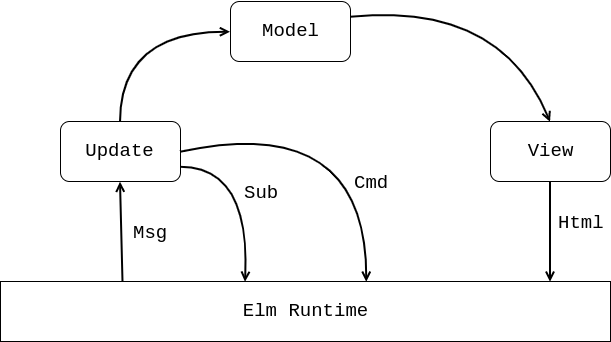
\includegraphics[width=0.6\textwidth]{images/elm_data_flow}
	\caption{Przepływ danych w języku Elm}
	\label{fig:elmFlow}
\end{figure}
\FloatBarrier
Niezależnie od rodzaju wykonywanej akcji, przepływ danych w języku Elm opiera się o podstawowe struktury zwane wiadomościami. Są to komunikaty zdefiniowane przez programistę w kodzie, które poza typem wiadomości mogą zawierać dane, na podstawie których aktualizowany jest modek. Silnik języka przesyła je wraz z aktualną wersją modelu do funkcji \lstinline{update}, która na podstawie rodzaju wiadomości oraz zawartych w niej danych aktualizuje model. Nowa wersja modelu zostaje następnie przekazana do funkcji \lstinline{view}, która buduje na jego podstawie pełną strukturę opisującą widok. Struktura ta, będąca obiektem typu \lstinline[style=elm-style]{Html}, skonstruowanym przy pomocy funkcji z implementacji Virtual DOM-u, jest następnie przesyłana do silnika Elma, który na jej podstawie aktualizuje drzewo DOM-u.

Elm posiada także dwa dodatkowe rodzaje komunikatów: komendy i subksrypcje. Te pierwsze odpowiadają za wysyłanie wiadomości obsługujących efekty uboczne, takie jak zapytania HTTP. Są one tworzone jako obiekty typu \lstinline[style=elm-style]{Cmd} posiadające w sobie typ wiadomości, jaka ma zostać wywołana. Obiekty takie są wysyłane równocześnie z modelem, jako część zwrotna funkcji \lstinline{update}, która wysyła model do funkcji odpowiadającej za budowę widoku, natomiast samą komendę przekazuje do silnika Elma. Silnik na podstawie podanej komendy wywołuje kolejną aktualizację modelu, jako wiadomość przekazując zawartość komendy. Subskrypcje natomiast, są sposobem na nasłuchiwanie zewnętrznych komunikatów takich jak ruchy myszy, zmiana adresu w przeglądarce, czy też zmiana jej rozmiaru. Są one zdefiniowane podczas uruchomienia aplikacji jako obiekty typu \lstinline[style=elm-style]{Sub}, które podobnie jak w przypadku komend posiadają w sobie typ wiadomości, która po nastąpieniu zewnętrznego zdarzenia jest wysyłana przez silnik języka do funkcji \lstinline{update}.

Prostota tak skonstruowanego przepływu danych pozwala na łatwą analizę działania aplikacji, niezależnie od jej rozmiaru. Programista nie jest zmuszony do zastanawiania się nad skomplikowaną architekturą, dzięki czemu jest w stanie szybko ustalić, w jaki sposób działa aplikacja. Prosty model aktualizacji danych oparty na komunikatach pozwala także na łatwe dodawanie nowych funkcjonalności, ponieważ wiąże się to z dodaniem nowego komunikatu, który jest definiowany niezależnie od poprzednio dodanych wiadomości.

\subsection{Komponent prezentacyjny i kontener}
Aby w ogóle zacząć temat jednokierunkowego przepływu danych w kombinacji React i Redux, trzeba wyjaśnić, czym są komponenty. W przeciwieństwie do Elma, który całą swoją strukturę opiera na funkcjach, React wprowadza specjalny rodzaj struktur umożliwiający zdefiniowanie wyświetlanych widoków.

W dokumentacji Reacta można znaleźć, że komponenty pozwalają podzielić interfejs na niezależne fragmenty wielokrotnego użytku i myśleć o każdym z fragmentów oddzielnie \cite{reactDocs}. Koncepcyjnie są one podobne do funkcji w JavaScript'cie. Przyjmują dowolne dane wejściowe, które zawarte są w pojedynczym obiekcie \lstinline{props}, a zwracają elementy Reacta, opisujące to, co powinno zostać wyświetlone. Fragmenty \ref{listing:statelesscomp} i \ref{listing:statefulcomp} przedstawiają dwa podstawowe sposoby tworzenia komponentów w React'cie: jako zwykła funkcja JavaScript oraz jako klasa ze standardu ECMAScript 6.
\newpage % Simple hack to remove first line of listing from page end
\begin{lstlisting}[style=JavaScript, caption=Funkcyjny komponent bezstanowy, label=listing:statelesscomp]
function Welcome(props) {
	return <h1>Hello, {props.name}</h1>;
}
\end{lstlisting}

\begin{lstlisting}[style=JavaScript, caption=Komponent stanowy jako klasa ECMAScript 6, label=listing:statefulcomp]
class Clock extends React.Component {
	constructor(props) {
		super(props);
		this.state = {date: new Date()};
	}
	render() {
		return (
			<div>
				<h1>It is {this.state.date.toLocaleTimeString()}.</h1>
			</div>
		);
	}
}
\end{lstlisting}
W pierwszym przypadku mamy do czynienia z komponentem funkcyjnym bezstanowym. Zgodnie z~jego nazwą charakteryzuje się brakiem lokalnego stanu oraz zapisem w formie funkcji przyjmującej jako argument obiekt \lstinline{props}, która zwraca elementy Reacta. Komponent tego typu nie pozwala także na zarządzanie jego cyklem życia, czy optymalizacją częstotliwości odświeżania. Aby skorzystać z tych funkcjonalności, należy użyć implementacji za pomocą klasy. Komponenty klasowe umożliwiają dodanie logiki do cyklu życia komponentu, co sprawia, że stają się one czymś więcej niż tylko obiektami opisującymi jakie elementy mają zostać wyświetlone na interfejsie użytkownika.

W kontekście połączenia Reacta i Reduxa często stosuje się inny podział, na komponenty prezentacyjne i kontenery. Różnią się one od siebie przede wszystkim tym, że kontenery są specjalnym rodzajem komponentów, które są świadome istnienia Reduxa. To one odpowiadają między innymi za pobranie danych ze stanu Reduxa, czy wysyłaniu akcji określających, w jaki sposób ma zostać zmieniony stan. Pobieranie danych w kontenerze się to poprzez użycie funkcji \lstinline{connect} ze specjalnej biblioteki \textit{react-redux} zawierającej kod wymagany do współpracy Reacta z Reduxem \cite{reduxDocs}. Funkcja \lstinline{connect} przyjmuje jako argument zdefiniowaną przez użytkownika funkcję określającą, który fragment stanu Reduxa ma zostać użyty w kontenerze. W przypadku komponentów prezentacyjnych jedynym źródłem danych są właściwości przekazane za pomocą obiektu \lstinline{props}, a jedynym możliwym sposobem na zmianę stanu są funkcje zwrotne, również przekazane jako część tego obiektu.

Powodem takiego podziału jest przede wszystkim oddzielenie komponentów widoku, które mogą być używane wielokrotnie i nie powinny zależeć od implementacji logiki odpowiadającej za pobieranie i zarządzanie danymi.

\subsection{Przepływ danych w Redux i lokalny stan komponentów}
Twórca Reduxa tworząc implementację biblioteki, inspirował się między innymi Elmem, w związku z~czym sposób przepływu danych występujący w bibliotece Redux jest bardzo zbliżony do implementacji z języka Elm, a pewne fragmenty Reduxa można porównać do części architektury \textit{Model-Update-View}.

Odpowiednikiem modelu jest pojedyncze drzewo stanu zawierające w sobie wszystkie dane aplikacji. Różnica występująca między implementacją w Elmie jest brak ograniczenia co do typu, co pozwala na dowolną modyfikację drzewa, bez zbędnej potrzeby wcześniejszego definiowania domyślnych wartości. 

Tak jak w Elmie podstawową strukturą służącą do komunikowania o aktualizacji jest wiadomość, tak w przypadku Reduxa wykorzystywane są akcje. Są to zwykłe obiekty JavaScriptu posiadające informacje o rodzaju komunikatu, a także mogące posiadać dane wykorzystane do aktualizacji. W przeciwieństwie do Elma Redux nie posiada dodatkowych komunikatów służących do obsługi efektów ubocznych czy zdarzeń z zewnątrz, co zmusza programistę do skorzystania z innych bibliotek obsługujących takie zdarzenia. Przykładem tutaj może być biblioteka \textit{redux-saga}, służąca do obsługi efektów ubocznych \cite{reduxSaga}, która dodatkowo wspiera komunikację z Reduxem.

Aktualizacja danych odbywa się za pomocą funkcji zwanych \textit{reducer'ami}. Są to funkcje bez efektów ubocznych, które na podstawie dotychczasowego stanu oraz akcji zwracają nowe, zaktualizowane drzewo stanu. W przypadku Reduxa programista nie jest zmuszony do tworzenia jednej funkcji odpowiadającej za wszystkie aktualizacje. Biblioteka udostępnia funkcję \lstinline{combineReducers}, przyjmującą wszystkie funkcje, które mają posłużyć jako reducer. Po przysłaniu akcji funkcja przesyła ją do wszystkich określonych w niej funkcji aktualizujących, a następnie zbiera wyniki do jednego obiektu.
\begin{figure}[h]
	\centering
	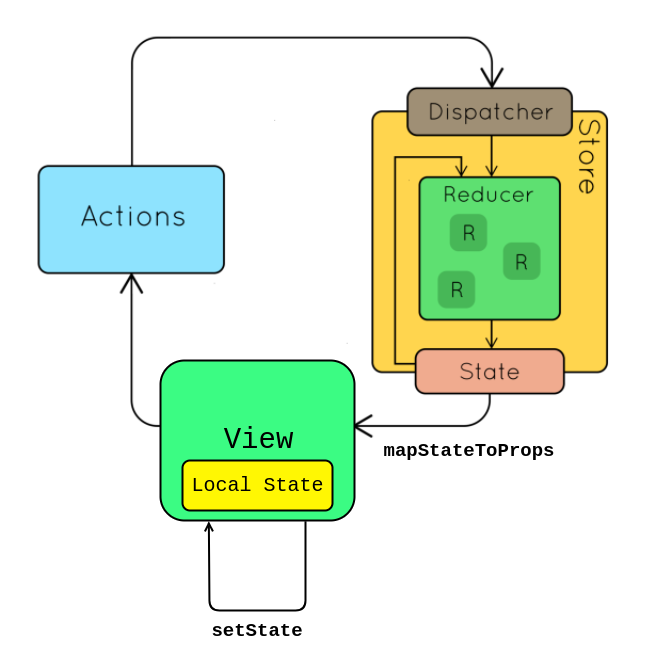
\includegraphics[height=0.38\textheight]{images/react_redux_data_flow}
	\caption{Przepływ danych w kombinacji React i Redux}
	\label{fig:reactReduxFlow}
\end{figure}
\FloatBarrier


\section{Niemutowalność obiektów}

\section{Biblioteki i menedżery pakietów}

\chapter{Porównanie dostępnych narzędzi}\label{chap:tools}
W tym rozdziale zostają opisane i porównane narzędzia wykorzystywane w czasie procesu budowy i rozwoju aplikacji stworzonych w języku Elm oraz kombinacji Reacta i Reduxa. Głównymi elementami na których jest skupiony rozdział są menedżery pakietów, narzędzia do statycznej analizy kodu oraz jego formatowania, a także narzędzia do monitorowania stanu w czasie działania aplikacji.

\section{Biblioteki i menedżery pakietów}
Ponieważ React, poza swoją specjalną składnią do opisywania komponentów widoku, składa się z~kodu JavaScriptu, to wykorzystywanym przez niego menedżerem pakietów jest npm. 

npm jest to menedżer pakietów dla języka JavaScript. Obecnie jest on także największym rejestrem oprogramowania, zawierający ponad 600 tysięcy pakietów kodu JavaScriptu z około 3 miliardami pobrań w ciągu jednego tygodnia \cite{whatIsNpm}. Menedżer pakietów npm składa się tak naprawdę z sieciowej bazy danych zawierającej publiczne, jak i płatne pakiety JavaScript oraz z klienta używanego w środowisku konsolowym. Rejest jest dostępny za pośrednictwem konsoli, a dostępne pakiety można przeglądać i~wyszukiwać za pomocą strony internetowej. 

Wszystkie pakiety instalowane w danej lokalizacji są zapisywane w specjalnym katalogu \lstinline{node_modules}, w którym znajdują się wszystkie zainstalowane pakiety oraz zależności wymagane do ich działania. Instalacja pakietów odbywa się poprzez polecenie \lstinline{npm install <nazwa_pakietu>}, co spowoduje instalację lokalną biblioteki w aktualnym folderze do katalogu \lstinline{node_modules}. Pakiet może być także zainstalowany globalnie, co umożliwia użycie go w dowolnym projekcie bez konieczności posiadania go bezpośrednio w każdym z nich.

Aby ułatwić zarządzanie lokalnie zainstalowanych pakietów, używany jest specjalny plik konfiguracyjny \lstinline{package.json}. Plik ten zawiera listę pakietów, od których zależy projekt, dla każdego z nich określając wersję pakietu, z których powinien korzystać projekt. Pozwala to na łatwe odtworzenie kompilacji, co znacznie upraszcza dzielenie kodu między programistami. Przykładową formę pliku można zobaczyć na fragmencie \ref{listing:package}.

\begin{minipage}{\linewidth}
\begin{lstlisting}[caption=Przykładowy plik package.json, tabsize=2, label=listing:package]
{
	"name": "elm-webpack-starter",
	"description": "Webpack setup for writing Elm apps",
	"version": "0.8.6",
	"license": "MIT",
	"author": "Peter Morawiec",
	"repository": {
		"type": "git",
		"url": "https://github.com/oszust002/elm-webpack-starter"
	},
	"scripts": {
		"start": "elm-css src/elm/Stylesheets.elm",
		"prebuild": "rimraf dist",
		"build": "webpack",
		"reinstall": "npm i && elm package install"
	},
	"devDependencies": {
		"autoprefixer": "^6.7.7",
		"elm-css": "^0.6.1"
	}
}
\end{lstlisting}
\end{minipage}
Aby uzyskać domyślny wersję pliku używa się komendy \lstinline{npm init --yes}, która na podstawie informacji zawartych w folderze projektu wygeneruje podstawowy plik konfiguracyjny zawierający pola:
\begin{itemize}
	\item name -- nazwa projektu. Domyślną wartością jest nazwa aktualnego katalogu
	\item version -- wersja projektu. Domyślnie zawsze jest to 1.0.0
	\item descripton -- krótki opis projektu. W przypadku istnienia pliku readme pobierana jest pierwsza linijka tego pliku, w przeciwnym wypadku jest tutaj wpisywany pusty ciąg znaków
	\item main -- wskazanie lokalizacji głównego pliku projektu. Domyślnie zawsze wskazywany jest plik \lstinline{index.js}
	\item scripts -- lista skryptów, które można wykonać przy pomocy polecenia \lstinline{npm run <nazwa_skryptu>}. Domyślnie tworzony jest pusty skrypt test
	\item keywords -- lista słów kluczowych, umożliwiająca znalezienie pakietu w rejestrze. Domyślnie jest ona pusta
	\item author -- informacje na tematu autora pakietu. Domyślnie pole to jest pustym ciągiem znaków
	\item license -- rodzaj licencji, która obejmuje pakiet. Domyślnie wpisywana jest licencja ISC.
\end{itemize}

Menedżer pakietów npm jest także często wykorzystywany przy tworzeniu projektów stworzonych w języku Elm. Jest on głównie wykorzystywany do instalowania pakietów pomocniczych, które pozwalają na interakcję z kodem Elma, taką jak generowanie kodu. Jednak projekty stworzone w języku Elm korzystają głównie z menedżera pakietów elm-package stworzonego przez twórcę Elma. Podobnie jak w~przypadku npm-a, elm-package składa się tak naprawdę na konsolowy interfejs służący do zarządzania pakietami w projekcie, oraz strony internetowej pozwalającej na przeglądanie poszczególnych pakietów \cite{elmPackage}. Niestety z powodu krótkiego istnienia języka oraz samego menedżera, liczba dostępnych pakietów, wynosząca niewiele ponad 1000 bibliotek, jest nieporównywalnie mała w stosunku do ilości pakietów wpisanych w rejestr npm-a. 

Podobnie jak w przypadku npm-a, menedżer pakietów dla języka Elm pozwala na łatwe zarządzanie pakietami wykorzystywanymi w projekcie. Odpowiednikiem pliku konfiguracyjnego jest tutaj plik \lstinline{elm-package.json}, znajdujący się w głównym katalogu projektu. Nowy plik konfiguracyjny jest tworzony w trakcie instalowania pierwszej biblioteki. Instalacja odbywa się za pomocą polecenia \lstinline{elm-package install <autor>/<nazwa_biblioteki> <wersja>}. Wymaganie autora biblioteki jest spowodowane tym, że menedżer pakietów dla języka Elm jest w tej chwili ograniczony wyłącznie do repozytoriów znajdujących się w serwisie GitHub. Wersja jest natomiast argumentem opcjonalnym, w przypadku niepodania go zostanie zainstalowana najnowsza wersja pakietu.
\begin{minipage}{\linewidth}
\begin{lstlisting}[caption=Przykładowy plik elm-package.json, tabsize=2, label=listing:elmPackage]
{
	"version": "1.0.0",
	"summary": "Example using `elm-webpack-loader`.",
	"repository": "https://github.com/moarwick/elm-webpack-starter.git",
	"license": "MIT",
	"source-directories": [ "src/elm" ],
	"exposed-modules": [],
	"dependencies": {
		"debois/elm-mdl": "8.1.0 <= v < 9.0.0",
		"elm-lang/core": "5.0.0 <= v < 6.0.0",
		"elm-lang/html": "2.0.0 <= v < 3.0.0",
		"rtfeldman/elm-css": "11.2.0 <= v < 12.0.0",
		"rtfeldman/elm-css-helpers": "2.1.0 <= v < 3.0.0"
	},
	"elm-version": "0.18.0 <= v < 0.19.0",
}
\end{lstlisting}
\end{minipage}
Na fragmencie \ref{listing:elmPackage} można zobaczyć przykładową formę pliku \lstinline{elm-package.json}. Analogicznie jak w~przypadku npm-a, znajdują się tutaj informacja na temat wersji projektu, krótkie podsumowanie, rodzaj licencji, czy w końcu lista pakietów wykorzystywanych w projekcie. Niestety pakiety mogą być instalowane tylko w sposób lokalny. To, co odróżnia zawartość pliku konfiguracyjnego dla elm-package od konfiguracji pakietów w npm-ie, jest między innymi brak nazwy pakietu, zastąpione adresem do repozytorium zawierającego paczkę. Nie ma tutaj także możliwości uruchamiania własnych skryptów, które mogłyby uprościć proces zarządzania aplikacją. Dodatkowo na końcu pliku znajduje się wersja wykorzystywanej implementacji języka Elm. Dzięki temu menedżer pakietów jest w stanie ustalić, które wersje bibliotek są kompatybilne z wykorzystaną wersją języka.

W przypadku pakietów języka Elm, wersje są istotnym aspektem ze względu na funkcjonalność obliczania zmian. Każda z bibliotek posiada wersję składającą się z trzech części: MAJOR, MINOR oraz PATCH. W pierwszym przypadku mamy do czynienia ze znaczną zmianą API, w której istniejące funkcjonalności zostały zmienione lub usunięte. W przypadku zmiany MINOR dodane zostały nowe funkcjonalności, bez wprowadzania jakichkolwiek zmian do już istniejących. Zmiana PATCH odpowiada za drobne poprawki nie zmieniające w żaden sposób API biblioteki. Menedżer pakietów przy pomocy polecenia \lstinline{elm-package bump} potrafi porównać wersję aktualną pakietu z wersją opublikowaną i na podstawie różnic automatycznie podnieść wersję aplikacji. W bardzo podobny sposób użytkownik, który chce sprawdzić różnice między konkretnymi wersjami danej biblioteki jest w stanie przy pomocy polecenia \lstinline{elm-package diff <autor>/<nazwa> <wersja1> <wersja2>} sprawdzić jakie dokładnie nastąpiły zmiany. Jest to możliwe dzięki wymuszeniu na osobach publikujących dodawania dokumentacji do projektu, która opisuje każdą z udostępnionych funkcjonalności. Obliczanie i sprawdzanie zmian pomiędzy wersjami to funkcja, która pomaga w zarządzaniu wykorzystywanymi wersjami bibliotek, a która niestety nie jest dostępny w przypadku menedżera pakietów npm.

\section{Statyczna analiza i formatowanie kodu}
W przypadku języka JavaScript narzędziami, które odpowiadają za statyczną analizę i formatowanie kodu źródłowego, są tak zwane lintery. Potrafią one wykryć potencjalne błędy, a także kod, który według zasad zdefiniowanych w danym linterze, jest trudny do utrzymania. Przykładami linterów są mięðzy innymi JSLint, JSHint, czy w końcu obecnie chyba najpopularniejszy z nich, ESLint. Ze względu na to, że ESLint jest jedynym narzędziem wspierającym składnię JSX wykorzystaną w React'cie, skupię się głównie na nim. Po stronie języka Elm trzeba rozróżnić dwa oddzielne narzędzia. Pierwszym jest po prostu kompilator Elma, który dzięki właściwościom języka potrafi przeprowadzać statyczną analizę kodu w czasie kompilacji. Drugim narzędziem natomiast jest pakiet elm-format, formatujący kod na podstawie oficjalnego przewodnika z zasadami poprawnego formatowania kodu w języku Elm~\cite{elmStyleGuide}. 

ESLint bazujący na wbudowanych zasadach poprawnego tworzenia kodu JavaScriptu potrafi wykryć błędy, które mogłyby doprowadzić do pojawienia się wyjątków po uruchomieniu aplikacji w przeglądarce. Na podstawie tychże zasad potrafi także ocenić jakość kodu stworzonego przez programistę i~zwrócić informację o tym, w jaki sposób można ten kod poprawić \cite{ESLint}. ESLint oferuje także elastyczność co do wykorzystywanych reguł. W każdej chwili, jeżeli programista nie chce, żeby dany fragment kodu był analizowany przez linter w kontekście jakiejś reguły, może wyłączyć ją za pomocą specjalnych przypisów dodanych w komentarzach. Pod tym względem zarówno kompilator języka Elm, jak i~biblioteka elm-format są o wiele bardziej restrykcyjne. Kompilator, przeprowadzając statyczną analizę kodu w czasie kompilacji, nie pozwoli na uruchomienie programu do momentu, w którym programista nie poprawi wskazanych fragmentów kodu. W przypadku elm-format sytuacja wygląda nieco inaczej. Biblioteka ta, zamiast analizować kod i wskazując niepoprawne miejsca programiście, automatycznie sama poprawia kod, opierając się na regułach dotyczących stylu opisanych w dokumentacji języka Elm \cite{elmStyleGuide}. Programista nie może zmienić reguł używanych przez elm-format, co narzuca wymóg tworzenia kodu w~jeden uniwersalny sposób.

O ile oczywistym jest to, że kompilator Elma jest narzędziem wbudowanym w język Elm, o tyle zarówno użycie ESLinta i biblioteki elm-format wymaga zewnętrznej konfiguracji. W obu przypadkach konfiguracja zaczyna się od zainstalowania bibliotek przy pomocy menedżera pakietów npm. Po tym kroku, biblioteka elm-format jest już gotowa do użycia, natomiast ESLint wymaga dodatkowej konfiguracji dla każdego projektu w którym ma być użyty. Odbywa się to za pomocą komendy \lstinline{eslint --init} generującej plik konfiguracyjny zawierający konfigurację jakie reguły mają zostać użyte w trakcie analizy kodu.

Choć doświadczeni programiści tworzący aplikacje internetowe używają powyższych narzędzi nawet o tym nie myśląc, to w przypadku osób zaczynających dopiero przygodę z programowaniem aplikacji internetowych, zdarza się nie wiedzieć o ich istnieniu. W przypadku języka Elm tracimy wyłącznie analizę i poprawę formatowania kodu. Kompilator jest wbudowanym narzędziem, które zawsze w przypadku błędów w kodzie, jest w stanie je znaleźć i przekazać użytkownikowi. Niestety w przypadku braku użycia ESLinta jesteśmy narażeni na wystąpienie błędów w trakcie działania programu. Aby pokazać na czym polega różnica, można rozważyć błąd, który jest popełniany bardzo często przez wielu programistów. Takim błędem są literówki. Niech w obu przypadkach występuje pole o nazwie \lstinline{fatalError}. W kontekście języka Elm pole to będzie częścią struktury modelu aplikacji, natomiast w implementacji Reacta będzie to jedno z pól właściwości dla komponentu.

\begin{minipage}{.45\textwidth}
	\begin{lstlisting}[style=elm-style,label = listing:elmmodel, numbers=left, stepnumber=1]
	type alias Model =
		{ field: String
		, fatalError: Bool
		}
	\end{lstlisting}
\end{minipage}\hfill
\begin{minipage}{.45\textwidth}
	\begin{lstlisting}[style=JavaScript,firstnumber=1,label=listing:reactprops]
	static propTypes = {
		field: React.PropTypes.string,
		fatalError: React.PropTypes.bool,
	};
	\end{lstlisting}
\end{minipage}

Aby wywołać błąd w obu przypadkach wystarczy odwołać się do pola \lstinline{fatalError}, jednak używając błędnie wpisanej nazwy \lstinline{fatalEror}. W przypadku implementacji w języku Elm, błąd zostanie wykryty już w czasie kompilacji. Rysunek \ref{fig:elmError} pokazuje komunikat wyświetlony przez kompilator, w~którym poza dokładnym miejscem wystąpienia błędu, programista otrzymuje podpowiedź o prawdopodobnej nazwie pola, której chciał użyć. Implementacja Reacta, w której nie skorzystano z ESLinta uruchomiła się nie podając żadnych komunikatów o błędach. Dopiero po wejściu na stronę internetową programista jest w stanie zauważyć że widok nie został załadowany, a sama informacja o występującym błędzie jest widoczna dopiero w konsoli deweloperskiej przeglądarki. Komunikat pokazany na rysunku~\ref{fig:reactError} jest stosem opisującym błąd, który mówi wprawdzie o nieistniejącej właściwości, jednak rozmiar komunikatu sprawia, że jest on mało czytelny. W przypadku większej ilości błędów, które mogą być dużo bardziej skomplikowane, programista może spędzić więcej czasu na szukaniu informacji o faktycznym błędzie, niż na samej jego poprawie.

\begin{figure}[h]
	\centering
	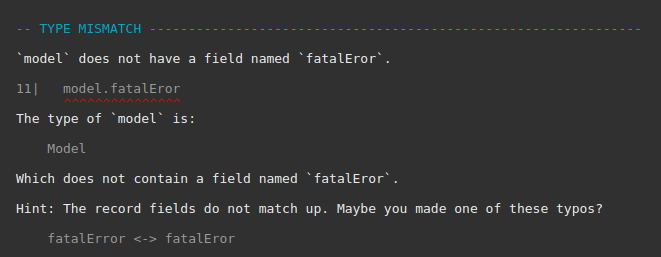
\includegraphics[width=0.9\textwidth]{images/elm_error}
	\caption{Komunikat kompilatora o nieistniejącym polu}
	\label{fig:elmError}
\end{figure}

\begin{figure}[h]
	\centering
	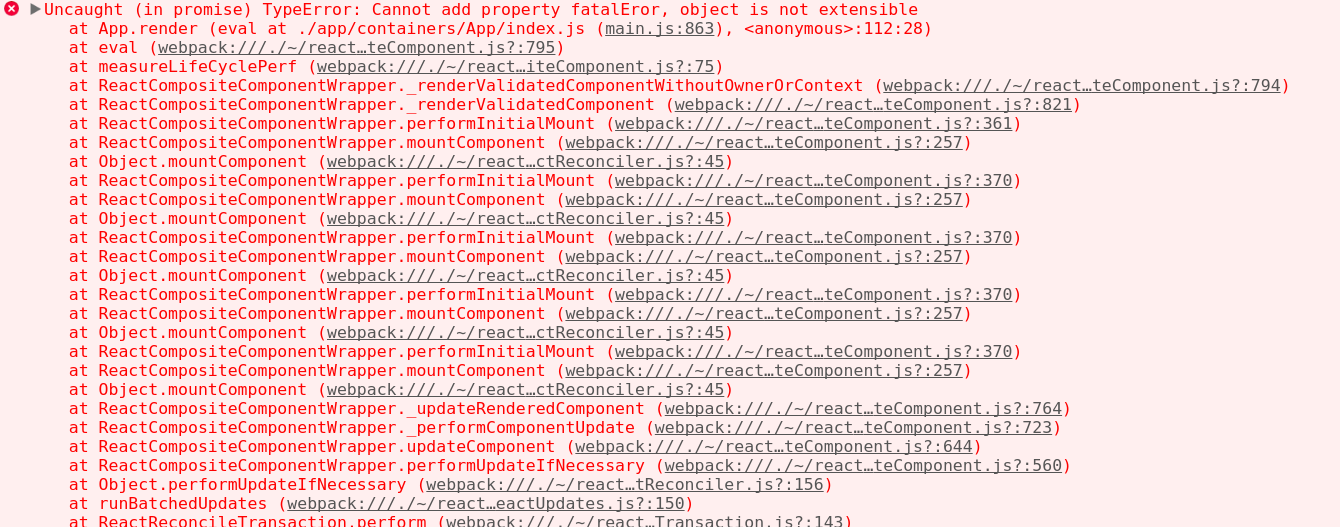
\includegraphics[width=0.9\textwidth]{images/react_error}
	\caption{Komunikat o błędzie w konsoli deweloperskiej przeglądarki Google Chrome}
	\label{fig:reactError}
\end{figure}

\section{Debugger języka Elm i Redux DevTools}
Sposób przepływu i aktualizacji danych w języku Elm i bibliotece Redux opiera się na komunikatach. Każda akcja, która w jakiś sposób modyfikuje stan aplikacji, jest odwzorowywana przez pojedynczą wiadomość. Takie podejście pozwala na łatwe monitorowanie stanu w czasie. Tym właśnie zajmują się narzędzia takie jak wbudowany w implementację języka Elm debugger oraz Redux DevTools.

Aby móc skorzystać z debuggera języka Elm, należy uruchomić program w trybie debug. To sprawia, że w prawym dolnym rogu widok aplikacji internetowej zostaje dołączona zakładka, która po kliknięciu przedstawia widok pokazany na rysunku \ref{fig:elmDebugger}. Po lewej stronie okna znajduje się lista wiadomości wysłanych od początku uruchomienia aplikacji w przeglądarce. Prawa strona natomiast prezentuje strukturę stanu w danym momencie działania aplikacji. Po kliknięciu jednej z wiadomości można zauważyć, że~z~prawej strony został pokazany stan z momentu tuż po zaaplikowaniu aktualizacji danych na podstawie tejże wiadomości. Stan ten jest aplikowany także do widoku, przez co programista jest w stanie zobaczyć, jak zmienia się widok w momencie wystąpienia konkretnego rodzaju komunikatu. Dodatkowo cały proces działania aplikacji można zapisać w formie pliku, co jest ogromnym ułatwieniem w procesie naprawiania błędów. Programista odpowiadający za dany fragment kodu ma możliwość wtedy wczytać cały proces z przekazanego mu pliku, dokładnie odtworzyć błąd, który wystąpił i znaleźć jego przyczynę.
\begin{figure}[h]
	\centering
	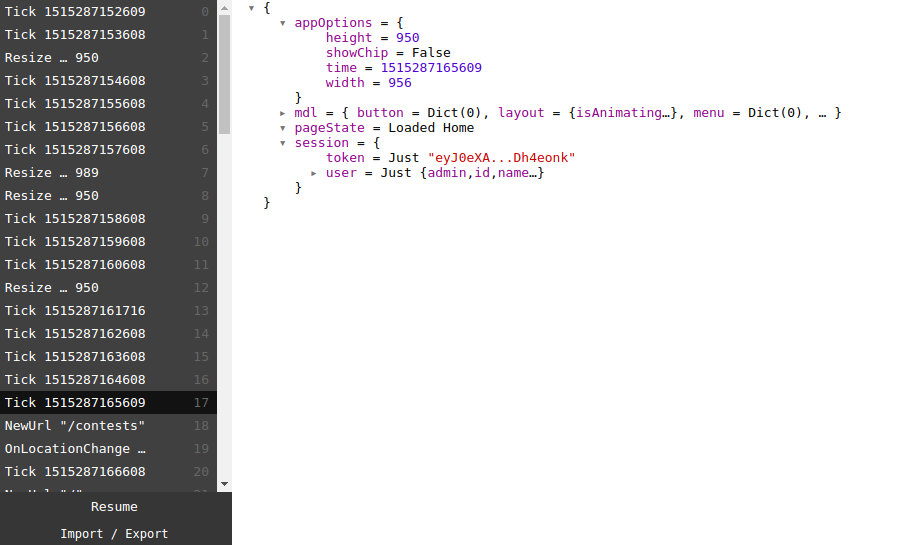
\includegraphics[width=\textwidth]{images/elm_debugger}
	\caption{Okno debuggera języka Elm}
	\label{fig:elmDebugger}
\end{figure}

Redux DevTools jest dodatkiem do przeglądarek takich jak Google Chrome czy Mozilla Firefox. Poza zainstalowaniem dodatku w przeglądarce należy dodać odpowiednie opcje we fragmencie kodu, w którym tworzony jest, przy pomocy funkcji Reduxa, stan całej aplikacji. Następnie po uruchomieniu aplikacji w narzędziach deweloperskich przeglądarki należy wejść w zakładkę \textit{Redux}, która pokaże nam okno pokazane na rysunku \ref{fig:reduxDevTools}. Od razu można zauważyć, że podobnie jak w~debuggerze Elma, po lewej stronie znajdują się akcje odpowiadające za aktualizację stanu, natomiast po prawej widać stan aplikacji w wybranym momencie. Można też tutaj, podobnie jak w debuggerze, zapisywać i wczytywać proces działania aplikacji. Jednak widać także, że Redux DevTools jest narzędziem znacznie bardziej rozbudowanym. Użytkownik może wybrać jeden z trzech sposobów wyświetlania drzewa stanu: jako drzewo danych tekstowych, wykres wizualizujący strukturę drzewa oraz bezpośrednie dane bez żadnej modyfikacji wizualnej. Poza widokiem stanu w danym momencie można także sprawdzić zawartość akcji, jaka została wtedy wysłana, a także spojrzeć na zmiany wprowadzone do stanu w skutek obsłużenia przychodzącej akcji. Dodatkową opcją jest też suwak pozwalający na przeglądanie zmian stanu w formie osi czasu. To, czego brakuje w narzędziu React DevTools w porównaniu do debuggera języka Elm to wizualizacja zmian na widoku aplikacji. Ponieważ narzędzie to jest tylko dodatkiem do przeglądarki, to nie ma ono bezpośredniego wpływu na widok aplikacji.

\begin{figure}[h]
	\centering
	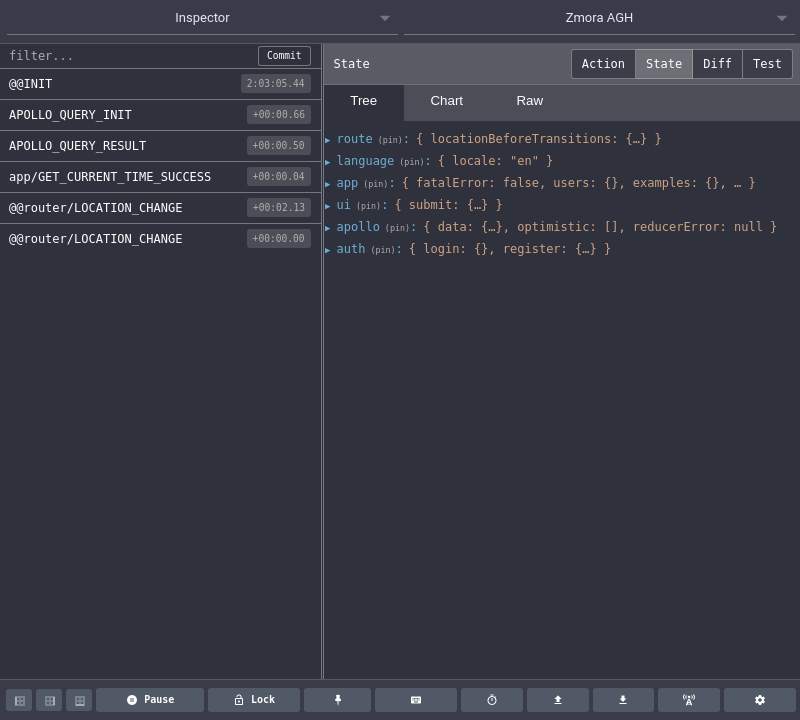
\includegraphics[width=0.9\textwidth]{images/redux_devtools}
	\caption{Okno dodatku Redux DevTools}
	\label{fig:reduxDevTools}
\end{figure}


\chapter{Implementacja} \label{chap:implementacja}
Rozdział ten skupia się na implementacji projektu, którym jest rekonstrukcja aplikacji internetowej stworzonej przy pomocy Reacta i Reduxa, w formie aplikacji napisanej w języku Elm. Opisane są w~nim założenia przyjęte w trakcie tworzenia aplikacji, uzyskany efekt oraz problemy napotkane w czasie implementacji.

\section{Założenia i uzyskany efekt}
Aplikacją, która została wybrana do rekonstrukcji w języku Elm, jest projekt stworzony przez grupę studentów uczelni Akademii Górniczo-Hutniczej. Aplikacja Zmora jest zautomatyzowaną platformą edukacyjną, skierowaną głównie do studentów kierunków informatycznych \cite{zmoraUi}. Jednym z jej elementów jest interfejs aplikacji internetowej stworzony głównie przy pomocy kombinacji Reacta i Reduxa.

Ze względu na rozbudowaną strukturę i ilość widoków dostępnych w aplikacji zostały wybrane tylko dwa. Jednym z nich jest strona główna aplikacji przedstawiona na rysunku \ref{fig:homOrg}, która poza górnym panelem oraz menu położonym z lewej strony, jest statyczną stroną, niepobierającą żadnych danych z~zewnątrz. Aby uwzględnić także komunikację z serwerem aplikacji, drugim wybranym widokiem jest strona logowania widoczna na rysunku \ref{fig:logOrg}. Czerwona linia oznacza te elementy widoku, które zostały uwzględnione przy rekonstrukcji. Znajdujący się po prawej stronie fragment odpowiedzialny za rejestrację nowych użytkowników nie został uwzględniony aby nie dodawać niepotrzebnych użytkowników.

\begin{figure}[h]
	\centering
	\begin{subfigure}{0.5\textwidth}
		\centering
		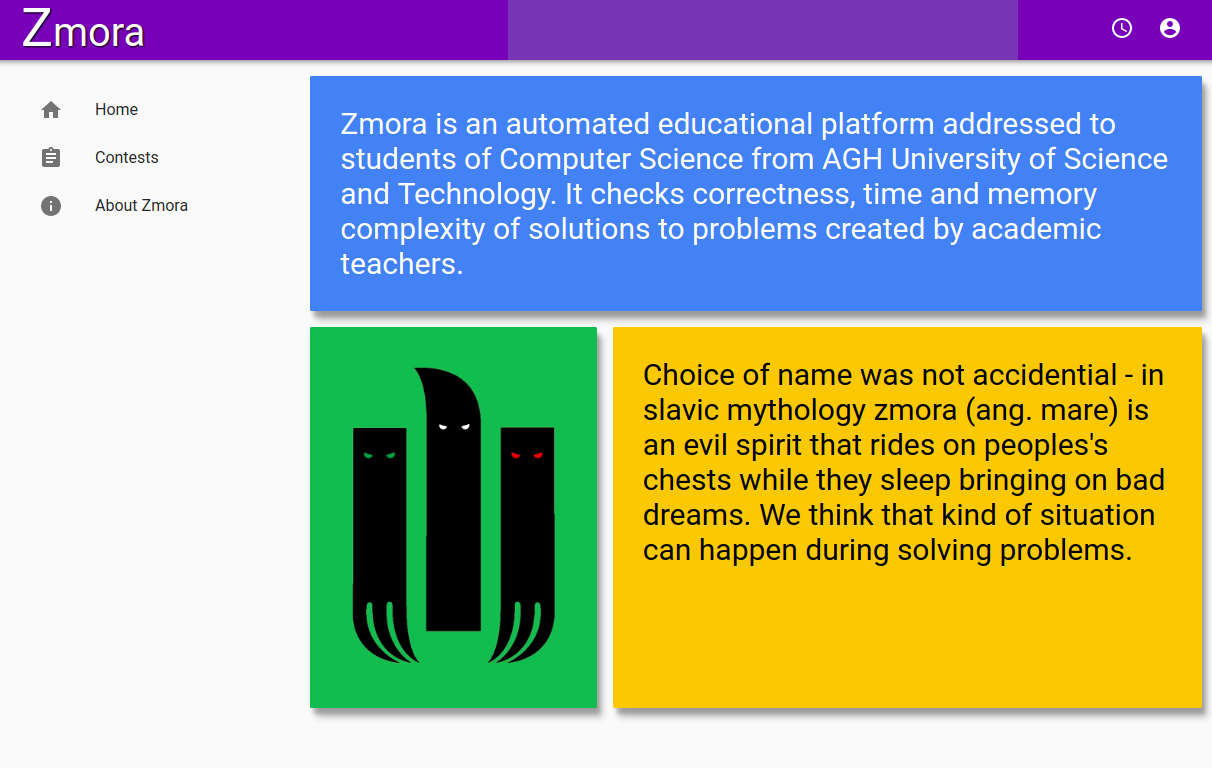
\includegraphics[width=0.9\linewidth]{images/homepage_zmora}
		\caption{Oryginalny widok strony głównej}
		\label{fig:homOrg}
	\end{subfigure}%
	\begin{subfigure}{0.5\textwidth}
		\centering
		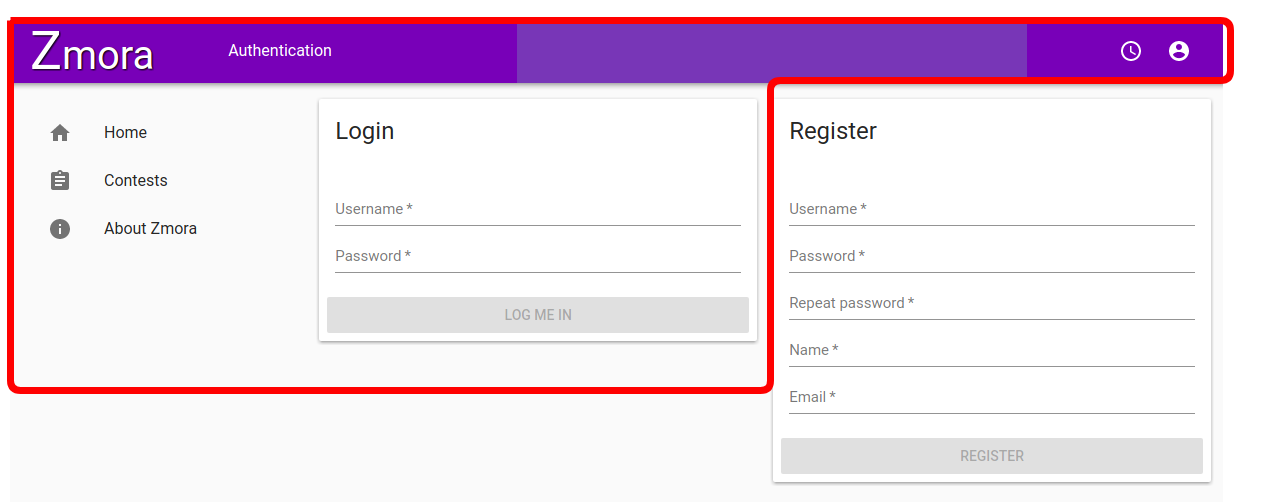
\includegraphics[width=0.9\linewidth]{images/login_zmora}
		\caption{Oryginalny widok strony logowania}
		\label{fig:logOrg}
	\end{subfigure}
	\label{fig:orgView}
	\caption{Widoki wybrane do zrekonstruowania}
\end{figure}

Ze względu na przyjęte w założeniach ograniczenia co do widoków, końcowy efekt mimo podobnego wyglądu w stosunku do oryginału różni się pod kilkoma względami. Menu boczne aplikacji znajdujące się na obu podstronach zgodnie z założeniami oryginalnej wersji aplikacji przenosi pod dokładnie te same adresy, jednak z powodu braku zaimplementowanych widoków zostaje wyświetlony dodatkowy widok stworzony specjalnie dla nie znalezionych stron. Porównując widok strony głównej w wersji oryginalnej oraz zrekonstruowanej przy pomocy języka Elm, ciężko dostrzec między nimi różnice. W~przypadku widoku strony logowania można zauważyć drobne przesunięcia obiektów w stosunku do oryginału. Wynikało to przede wszystkim z różnicy używanych bibliotek. W trakcie tworzenia rekonstrukcji jedynymi bibliotekami odpowiadającymi za widok były pakiety udostępnione przez menedżer pakietów elm-package, oraz style w postaci plików CSS.
\begin{figure}[h]
	\begin{subfigure}{0.5\textwidth}
		\centering
		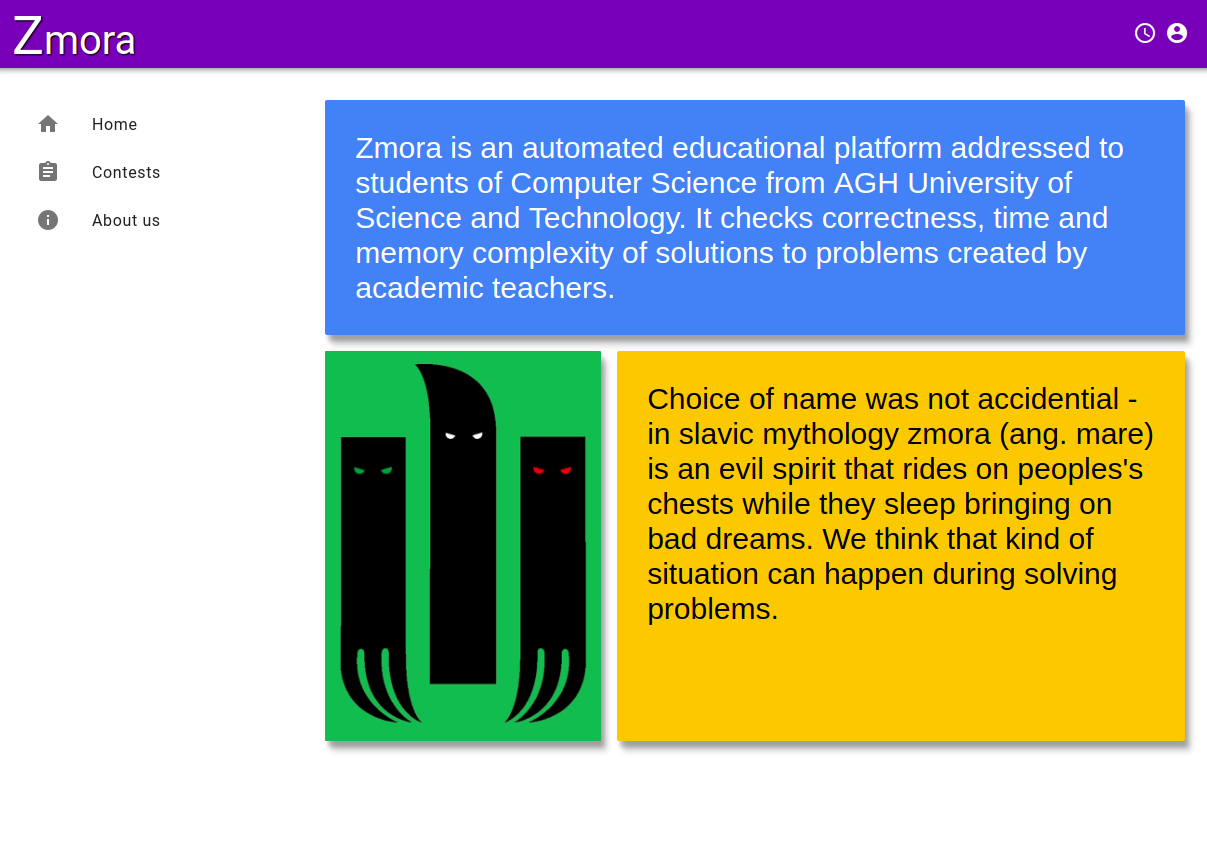
\includegraphics[width=0.9\linewidth]{images/homepage_elm}
		\caption{Zrekonstruowany widok strony logowania}
		\label{fig:homElm}
	\end{subfigure}%
	\begin{subfigure}{0.5\textwidth}
		\centering
		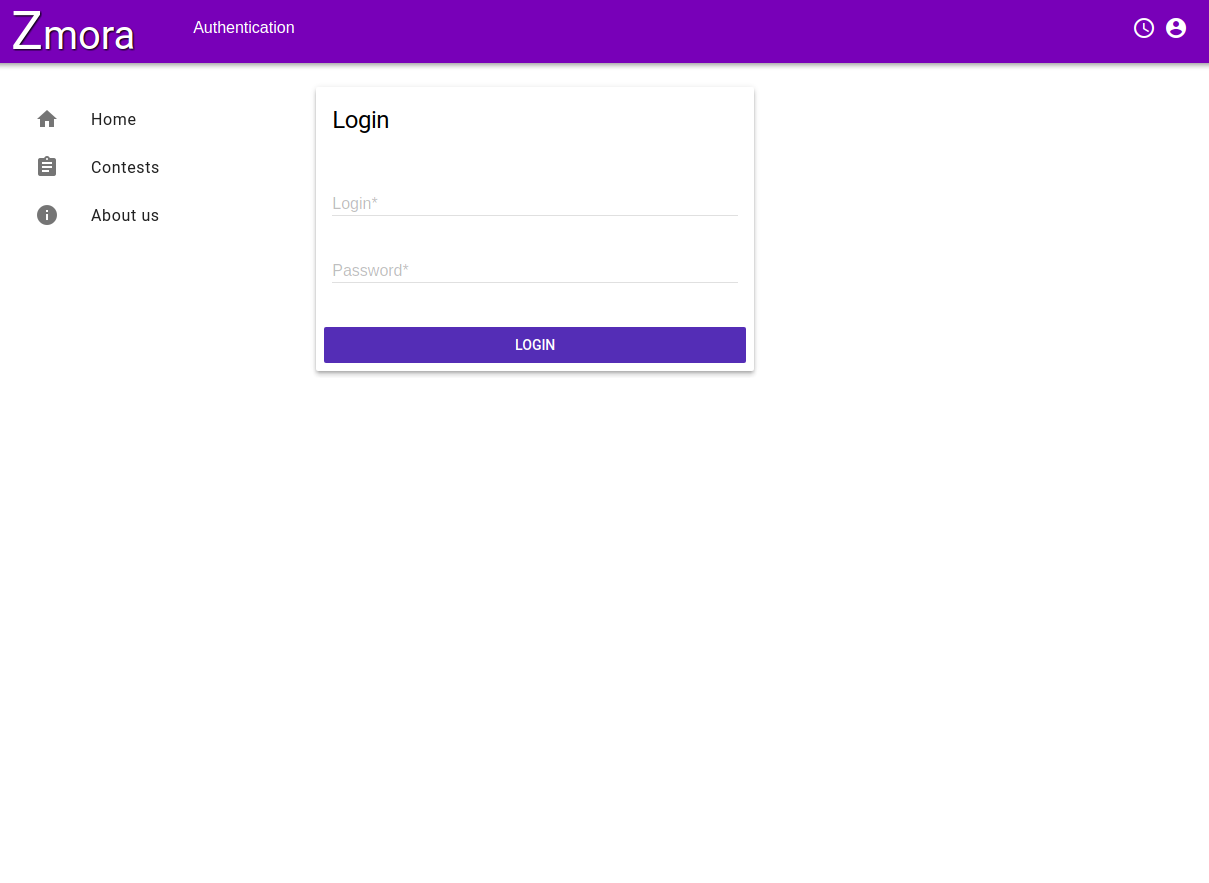
\includegraphics[width=0.9\linewidth]{images/login_elm}
		\caption{Zrekonstruowany widok strony logowania}
		\label{fig:logElm}
	\end{subfigure}
	\caption{Zrekonstruowane widoki stworzone przy pomocy języka Elm}
	\label{fig:elmView}
\end{figure}

\section{Napotkane problemy}
Głównym problemem, jaki został napotkany podczas rekonstrukcji aplikacji była dostępność bibliotek służących do budowania widoku oraz obsługi danych. Widok aplikacji w przypadku oryginału był budowany za pomocą komponentów biblioteki Material-UI, która implementuje styl Material Design. Jest to styl graficzny stworzony przez firmę Google, którego założeniem była prostota, czytelność i~łatwość dostosowania do różnych płaszczyzn. Niestety, menedżer pakietów, z którego korzystał Elm, oferował jedynie bibliotekę będącą portem uboższej wersji Material Designa o nazwie Material Design Lite. Spowodowało to, że proste komponenty, takie jak górna belka aplikacji, które w oryginalnej implementacji zajmowały kilka linijek kodu, w zrekonstruowanej wersji stawały się ogromnymi elementami, które trzeba było modyfikować za pomocą własnych stylów.

Dużym problemem było także znalezienie biblioteki do obsługi danych. Serwer aplikacji oferuje zarządzanie danymi poprzez zapytania języka GraphQL. W przypadku oryginalnej implementacji została użyta biblioteka stworzona przez twórców API, z którego korzystał serwer. Będąc pakietem specjalnie skonstruowanym dla Reacta, umożliwiała szybkie i proste definiowanie zapytań przy pomocy składni języka GraphQL. Aby skorzystać z podobnej funkcjonalności w zrekonstruowanej wersji aplikacji, wykorzystano oferowaną w menedżerze pakietów npm bibliotekę, która na podstawie plików zawierających treść zapytań w języku GraphQL oraz konfiguracji typów pobieranej z serwera, generowała pliki z~kodem Elma, zawierające funkcje oraz typy umożliwiające korzystanie z zapytań do serwera wewnątrz kodu aplikacji. Niestety API wystawione przez serwer nie było w pełni uwzględnione w konfiguracji serwera. Dane, które były zwracane przez serwer, były opakowywane w dodatkowy obiekt, co powodowało, że przy próbie dekodowania danych do typów języka Elm operacja kończyła się niepowodzeniem. Jedynym możliwym rozwiązaniem okazało się zmodyfikowanie biblioteki generującej moduły Elma w~taki sposób, aby niezależnie od podanego zapytania ostateczne dane były opakowywane w dodatkowy typ.

Inną trudnością, która wystąpiła podczas rekonstrukcji oryginalnych widoków, było zaprojektowanie modelu danych. W przeciwieństwie do kombinacji Reacta i Reduxa, które bazując na JavaScript'cie nie są ograniczone przez typy i mogą modyfikować w każdej chwili stan, dodając do niego kolejne pola. W~przypadku Elma model danych jest ustalony z góry przez silne typowanie, przez co model musiał być zaprojektowany tak, aby uwzględnić każdy przypadek danych otrzymywanych od serwera. Dodatkowym utrudnieniem było trzymanie opcji dotyczących widoku razem z danymi aplikacji. To wszystko powodowało, że stan aplikacji stawał się po jakimś czasie obiektem o skomplikowanej strukturze, który dodatkowo był ograniczony przez typy, co wymuszało przewidzenie wszystkich możliwych sytuacji zmiany stanu bez możliwości praktycznego przetestowania aplikacji.
\chapter{Podsumowanie} \label{chap:podsumowanie}
Celem tej pracy było porównanie dwóch sposobów budowania i rozwoju aplikacji internetowych: przy pomocy języka Elm oraz kombinacji bibliotek React.js i Redux. 
Obie technologie miały zostać porównane pod względem architektury, udostępnianych funkcjonalności, wydajności aplikacji oraz dostępnych bibliotek i narzędzi. Dodatkowo w ramach praktycznego porównania miała zostać przygotowana aplikacja stworzona przy pomocy języka Elm, która odwzorowywała pewną część innej aplikacji napisanej przy pomocy bibliotek React i Redux. 

Pomimo porównania języka do dwóch bibliotek, okazało się, że pod względem architektonicznym połączenie Reacta i Reduxa jest bardzo podobne do podejścia stosowanego w języku Elm. Te same funkcjonalności zaimplementowane w różny sposób pozwoliły na porównanie, która z technologii może być oceniana jako lepsza w kontekście tworzenia aplikacji internetowych. Sporym czynnikiem mającym wpływ na ocenę obu technologii były problemy, które pojawiły się podczas realizacji praktycznej części pracy w formie projektu. 

Analiza architektury języka Elm oraz bibliotek React i Redux pokazała, że w zależności od wybranego kontekstu, na podstawie którego te technologie są porównywane, decyzja o tym, która z nich jest lepsza, potrafi być zmienna. 

Pod względem szybkości wyświetlania widoku zdecydowanym zwycięzcą jest Elm, który dzięki optymalizacjom zawartym w swoim silniku do budowy Virtual DOM-u jest w stanie pominąć niektóre klatki, które i tak nie są widoczne dla użytkownika. Argumentem stojącym za wyborem Elma jest też to, że pewne elementy, takie jak narzędzia do analizy kodu i procesu działania aplikacji są wbudowane bezpośrednio w sam silnik języka, w przeciwieństwie do Reacta i Reduxa, które muszą korzystać z zewnętrznych rozwiązań, o których trzeba pamiętać. Część porównywanych elementów architektury nie pozwala jednak na bezpośrednie wybranie lepszej technologii, ponieważ każdy programista preferuje inne podejście do tworzenia oprogramowania. Mowa tu o elementach takich jak wybór między silnym a~dynamicznym typowaniem, preferencji trzymania wszystkich danych w jednym miejscu, a możliwością skorzystania z lokalnego stanu oferowanego przez komponenty, czy chociażby wybór między komponentami zawierającymi własny cykl życia a funkcjami w Elmie działającymi za każdym razem w ten sam sposób, bez efektów ubocznych. Aspektem, który stawia Reacta i Reduxa na wygranej pozycji jest przede wszystkim ich popularność oraz dostępność bibliotek. Z racji tego, że są to po prostu biblioteki języka JavaScript, mogą one korzystać bezpośrednio z każdego dostępnego pakietu stworzonego przy pomocy tego języka, który jest obecnie najpopularniejszym językiem do budowania aplikacji internetowych.

Podsumowując całą pracę, nie można wybrać, która z porównywanych technologii jest lepsza. Zarówno język Elm, jak i kombinacja Reacta i Reduxa mają swoje zalety, a także wady. Trzeba zwrócić także uwagę na to, że porównując technologie wykorzystywane do tworzenia aplikacji internetowych, wyników takiego porównania nie można brać pod uwagę przez dłuższy okres. Rynek tworzenia oprogramowania webowego jest jednym z najczęściej i najszybciej zmieniających się gałęzi programowania. Być może za kilka lat zmieni się on na tyle, że jego popularność wzrośnie i całkowicie wyprze używane obecnie biblioteki. 



% itd.
% \appendix
% \include{dodatekA}
% \include{dodatekB}
% itd.
\printbibliography

\end{document}
